%====================================================================================================
% ?????
%====================================================================================================
% TCC
%----------------------------------------------------------------------------------------------------
% Autor				: Jasane Schio
% Orientador		: Gedson Faria
% Co-Orientador		: Angelo Darcy
% Instituição 		: UFMS - Universidade Federal do Mato Grosso do Sul
% Departamento		: CPCX - Sistema de Informação
%----------------------------------------------------------------------------------------------------
% Data de criação	: 01 de Outubro de 2015
%====================================================================================================
% 
\chapter{Testes e Resultados} 
\section{Considerações Iniciais}
Este capítulo está divido em duas seções, nas quais estão presente os testes realizados bem como se discute os mesmos. Primeiramente se descreve o processo de calibração de cores bem como a preparação do campo, configuração de imagem, e seu resultado. Em seguida são apresentados os resultados dos testes executados com o arquivo gerado na calibração. Os resultados foram separados em Cores Comuns e Cores com Problemas. Por último se faz uma análise geral dos resultados obtidos.


 Para realização dos testes foi desenvolvido um aplicativo Desktop para fazer a leitura do arquivo gerado pela calibração, que possibilita a exibição de uma imagem contendo os objetos de acordo com a cor selecionada, por meio de um menu de escolha. Sendo assim possível a análise dos resultados obtidos para cada uma das cores. 
 
  O teste foi feito de uma só vez, porém sua análise está separada em duas partes. A primeira parte Cores Comuns, são as cores que não apresentam problema devido a semelhança com outras cores, na qual estava presente as cores amarelo, azul, verde, rosa, roxo. Na segunda parte estão presente as Cores com Problemas, que contem as cores vermelho e laranja. 
 
 A seguir está detalhado o processo de calibração, bem como a maneiro com que o mesmo ocorreu. Após a explanação da calibração estão exposto os resultados deste teste e a validação de cada um.
\section{Calibração}
A calibração descrita ocorreu no dia 19 de Agosto de 2016, entre 17:36 e 17:39.
A rotina de calibração do sistema, já descrita no Capítulo 3, envolve primeiramente uma aquisição da imagem do campo vazio, como visto na Figura \ref{campovazio}.
\begin{figure}[H]
		\centering
		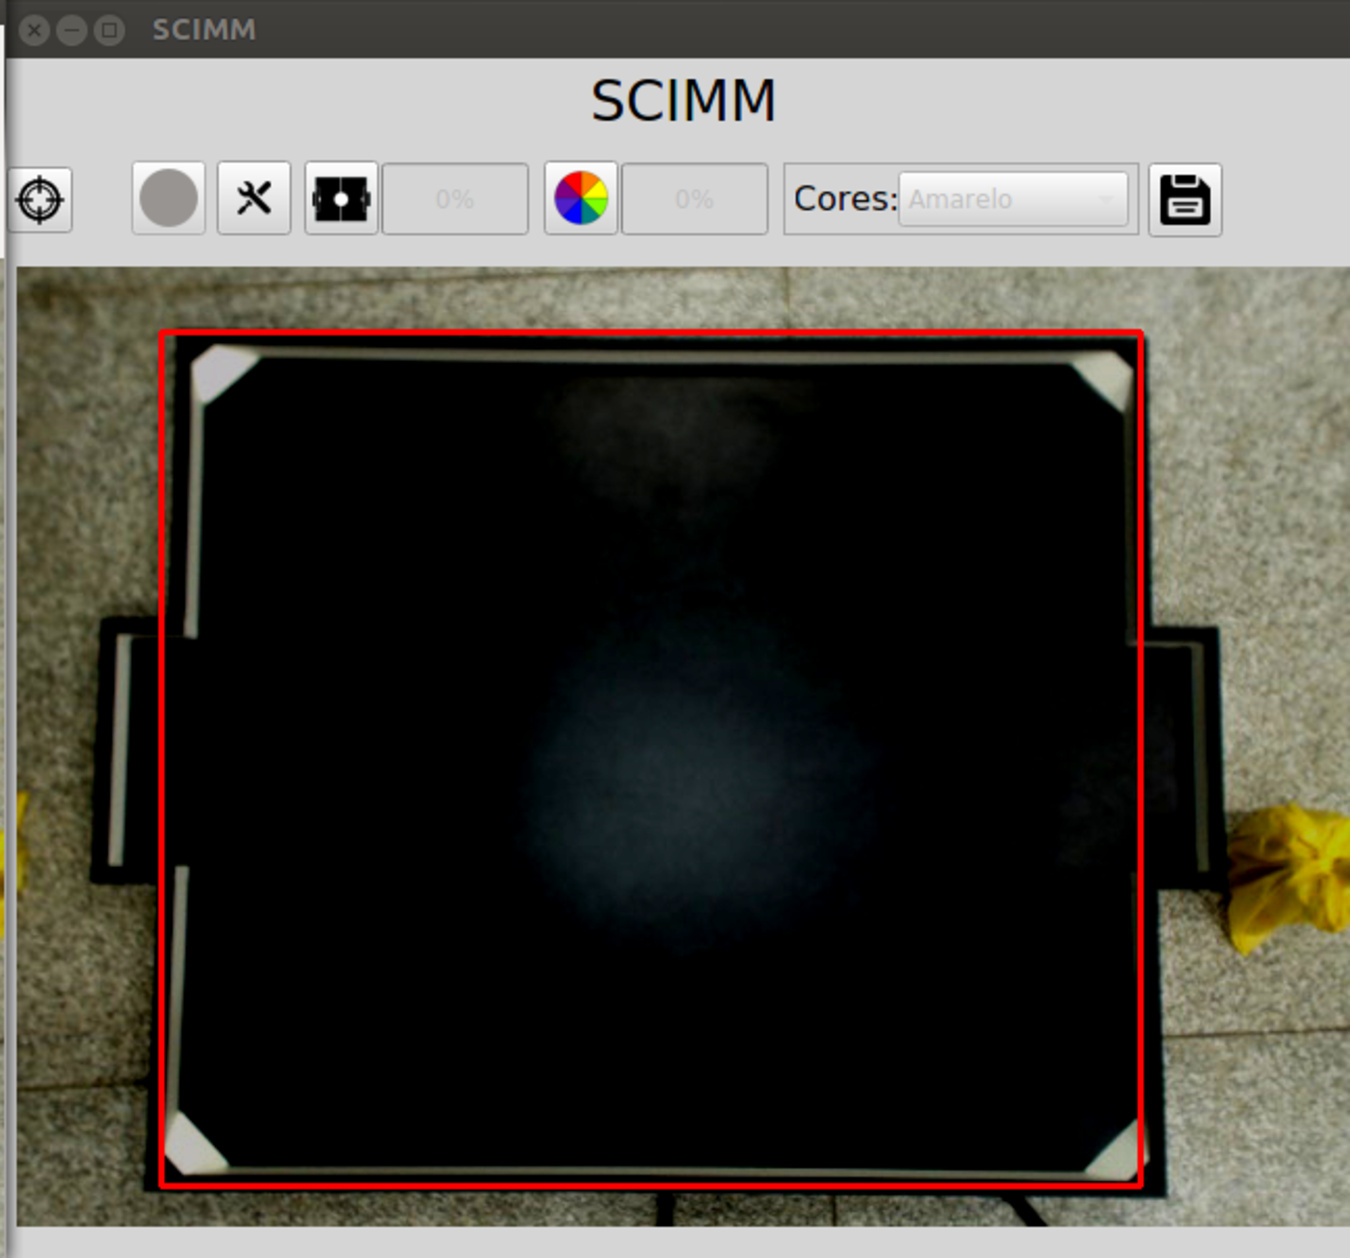
\includegraphics[width=0.45\textwidth]{fundoteste.pdf}
		\caption{Imagem do fundo com a seleção de campo}
		\label{campovazio}
	\end{figure}
Após ter o campo identificado pelo sistema, deve-se dispor sobre o campo os objetos coloridos, com as cores que se deseja obter o intervalo. É preferido que se usem tiras coloridas, pois quanto maior o tamanho da tira de cor, maior sera o espectro de cores que será analisado, assim sendo possível uma melhor qualidade de calibração.
Neste teste foram dispostos no campo tiras coloridas com largura entre \textit{17cm} e \textit{40cm} e altura entre \textit{5,5cm} e \textit{10,5cm}. Cada cor com 3 tiras, uma vez que o campo foi separado em três partes, para exemplificar diferentes luminosidades. A disposição das tiras pode ser vista na Figura \ref{fig:objetodispostos}.
	
	\begin{figure}[H]
%\begin{minipage}[H]{0.34\linewidth}
%\hspace{0.5cm}
\centering
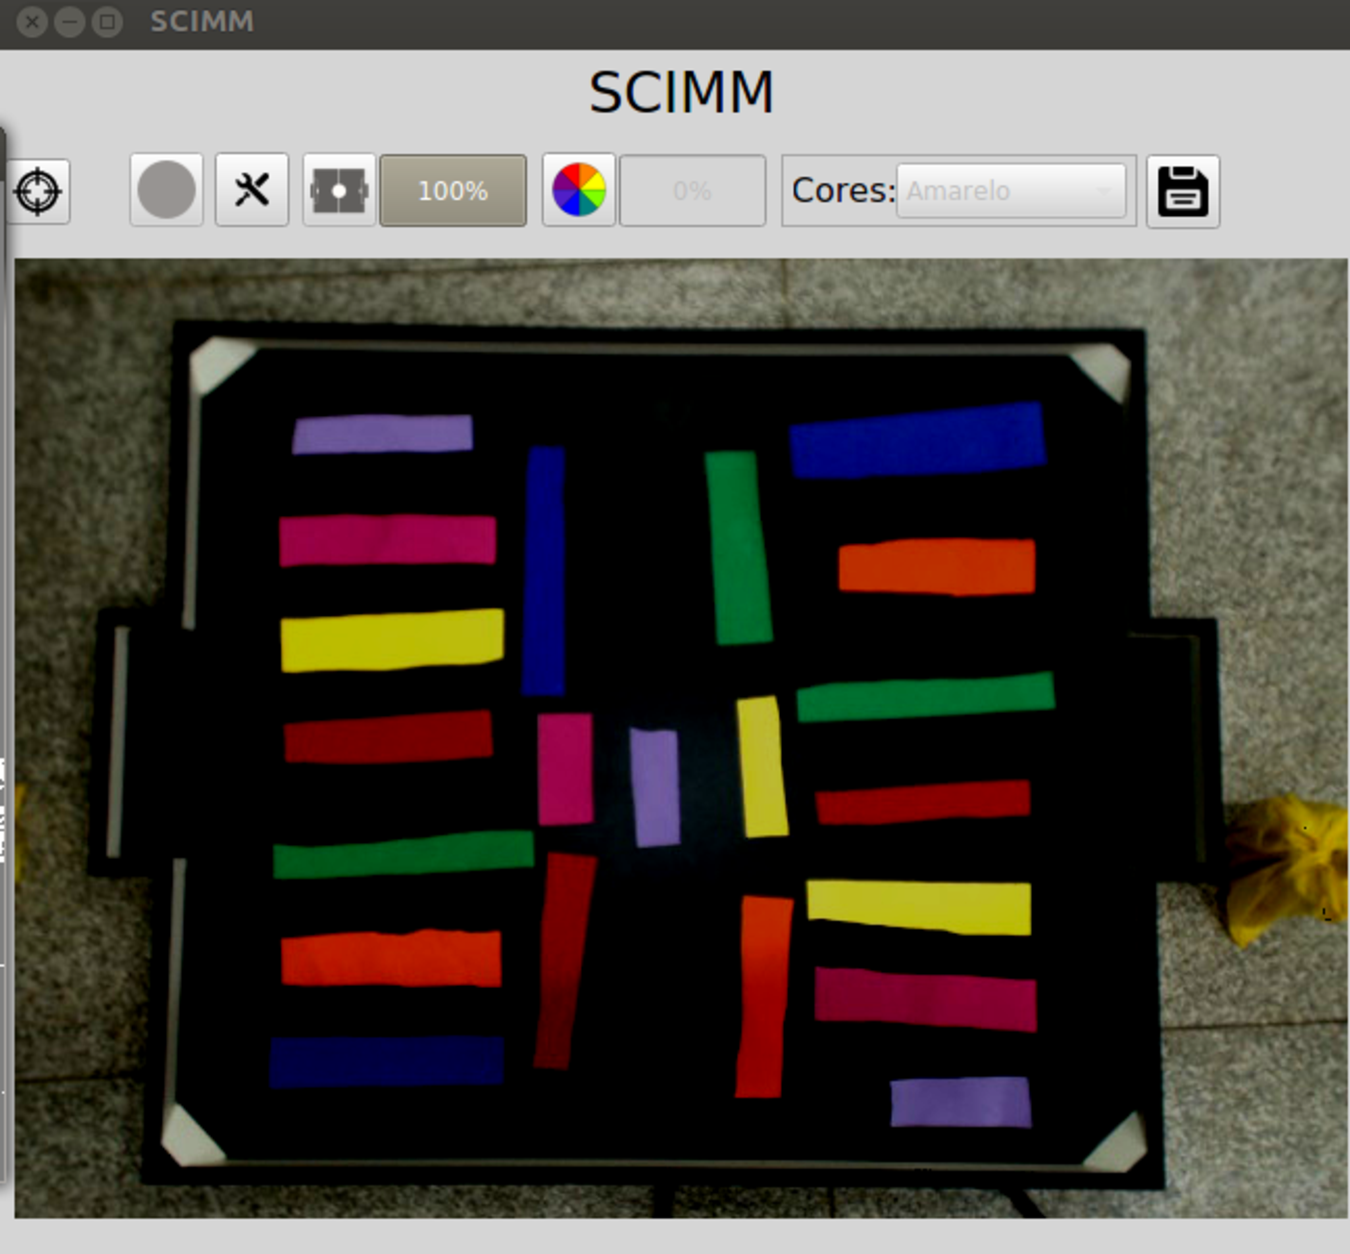
\includegraphics[width=0.45\textwidth]{objetosdispostos.pdf}
\caption{Objetos dispostos no campo para calibração}
\label{fig:objetodispostos}
%\end{minipage}
%\hspace{0.5cm}
%\begin{minipage}[H]{0.40\linewidth}
%\centering
%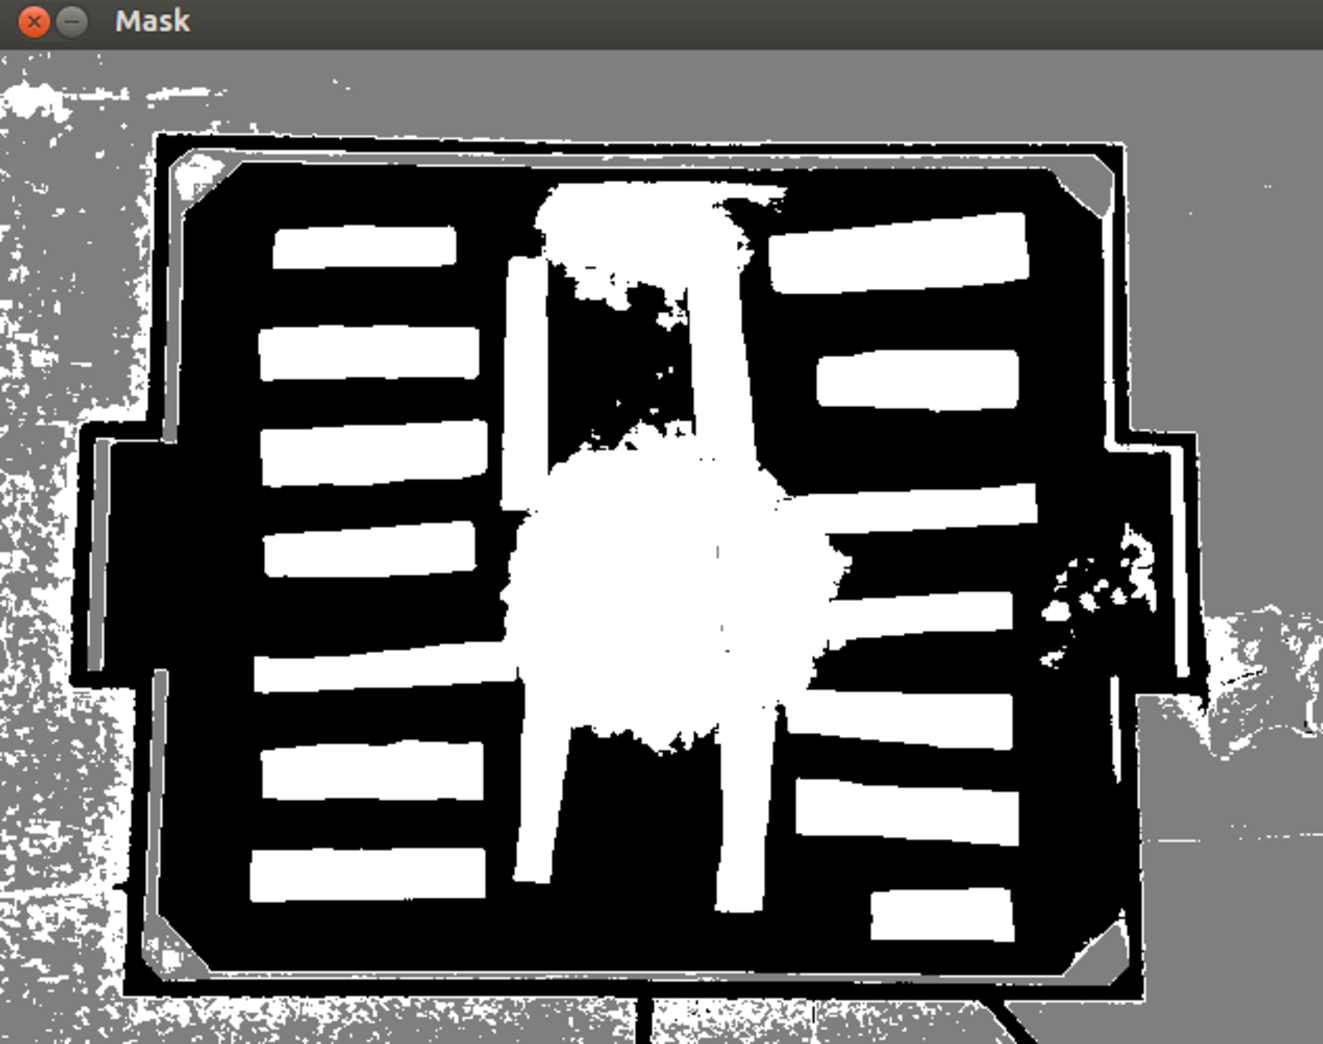
\includegraphics[width=\textwidth]{mascaragerada.pdf}
%\caption{Mascara gerada a partir da subtração de fundo}
%\label{fig:mascaragerada}
%\end{minipage}
\end{figure}	
	
Como resultado da rotina de calibração foi gerado um arquivo .arff contendo 14 linhas. A Tabela \ref{tab:arquivo} possui uma explicação sobre o arquivo gerado. A primeira coluna da tabela designa a linha contida no arquivo, a segunda coluna possui o conteúdo existente na arquivo, na última coluna está a descrição do conteúdo da linha do arquivo.
	\begin{table}[H]
\centering 
\begin{tabular}{l|c|c}
Linha & Conteúdo & Descrição  \\% Note a separação de col. e a quebra de linhas
\hline                               % para uma linha horizontal
 1& 21.50.50  &   Valor mínimo da cor Amarelo \\ \hline  
2& 30.255.255  &  Valor máximo da cor Amarelo \\  \hline 
3& 92.100.100  &   Valor mínimo da cor Azul \\  \hline 
4& 120.255.255  &  Valor máximo da cor  Azul \\  \hline 
5& 62.30.100 &  Valor mínimo da cor Verde \\  \hline 
6& 90.255.255  &  Valor máximo da cor Verde \\  \hline 
7& 169.100.100  &  Valor mínimo da cor Vermelho \\  \hline 
8& 179.255.255  &  Valor máximo da cor Vermelho \\   \hline 
9& 0.100.100  &  Valor mínimo da cor Laranja \\  \hline 
10& 20.255.255 &  Valor máximo da cor  Laranja \\  \hline 
11& 161.100.100 &  Valor mínimo da cor Rosa \\  \hline 
12& 168.255.255 &   Valor máximo da cor Rosa \\  \hline 
13& 126.30.30 &  Valor mínimo da cor Roxo \\  \hline 
14& 160.255.255 &  Valor máximo da cor Roxo \\  \hline 

\end{tabular}
\caption{Os valores de HSV estão separados por pontuação, H.S.V}
\label{tab:arquivo}
\end{table}





 \section{Testes}
O teste aqui descrito ocorreu dia no 26 de Agosto de 2016, entre à 13:28 e 16:28.
Para elaboração do teste optou-se por dividir o campo no maior numero de partes possíveis, e ainda assim que essas partes coubessem todas as 7 cores usadas. Essa divisão foi feita para simular as cores em todas as partes possíveis do campos. O campo foi divido em 15 partes de \textit{29cm x 41cm}, nomeadas alfabeticamente de A a O, como mostra a Figura \ref{campodivisao}.

\begin{figure}[H]
		\centering
		\includegraphics[width=0.3\textwidth]{campodivisao.pdf}
		\caption{Divisão do campo em quinze partes nomeadas alfabeticamente.}
		\label{campodivisao}
	\end{figure}
	
Cada uma das partes do campo continha as sete cores. Vermelho, Amarelo e Azul na primeira linha. Verde, Roxo, Laranja e Rosa na segunda. As cores estão distantes verticalmente \textit{6cm}. Na primeira linha a distância horizontal entre as cores é de \textit{7,25cm} e na segunda linha esta distancia é de \textit{5cm}. Um  melhor detalhamento da disposição das cores é visto nas Figuras \ref{fig:figure1} e \ref{fig:figure2}.


\begin{figure}[H]
\begin{minipage}[b]{0.45\linewidth}
\centering
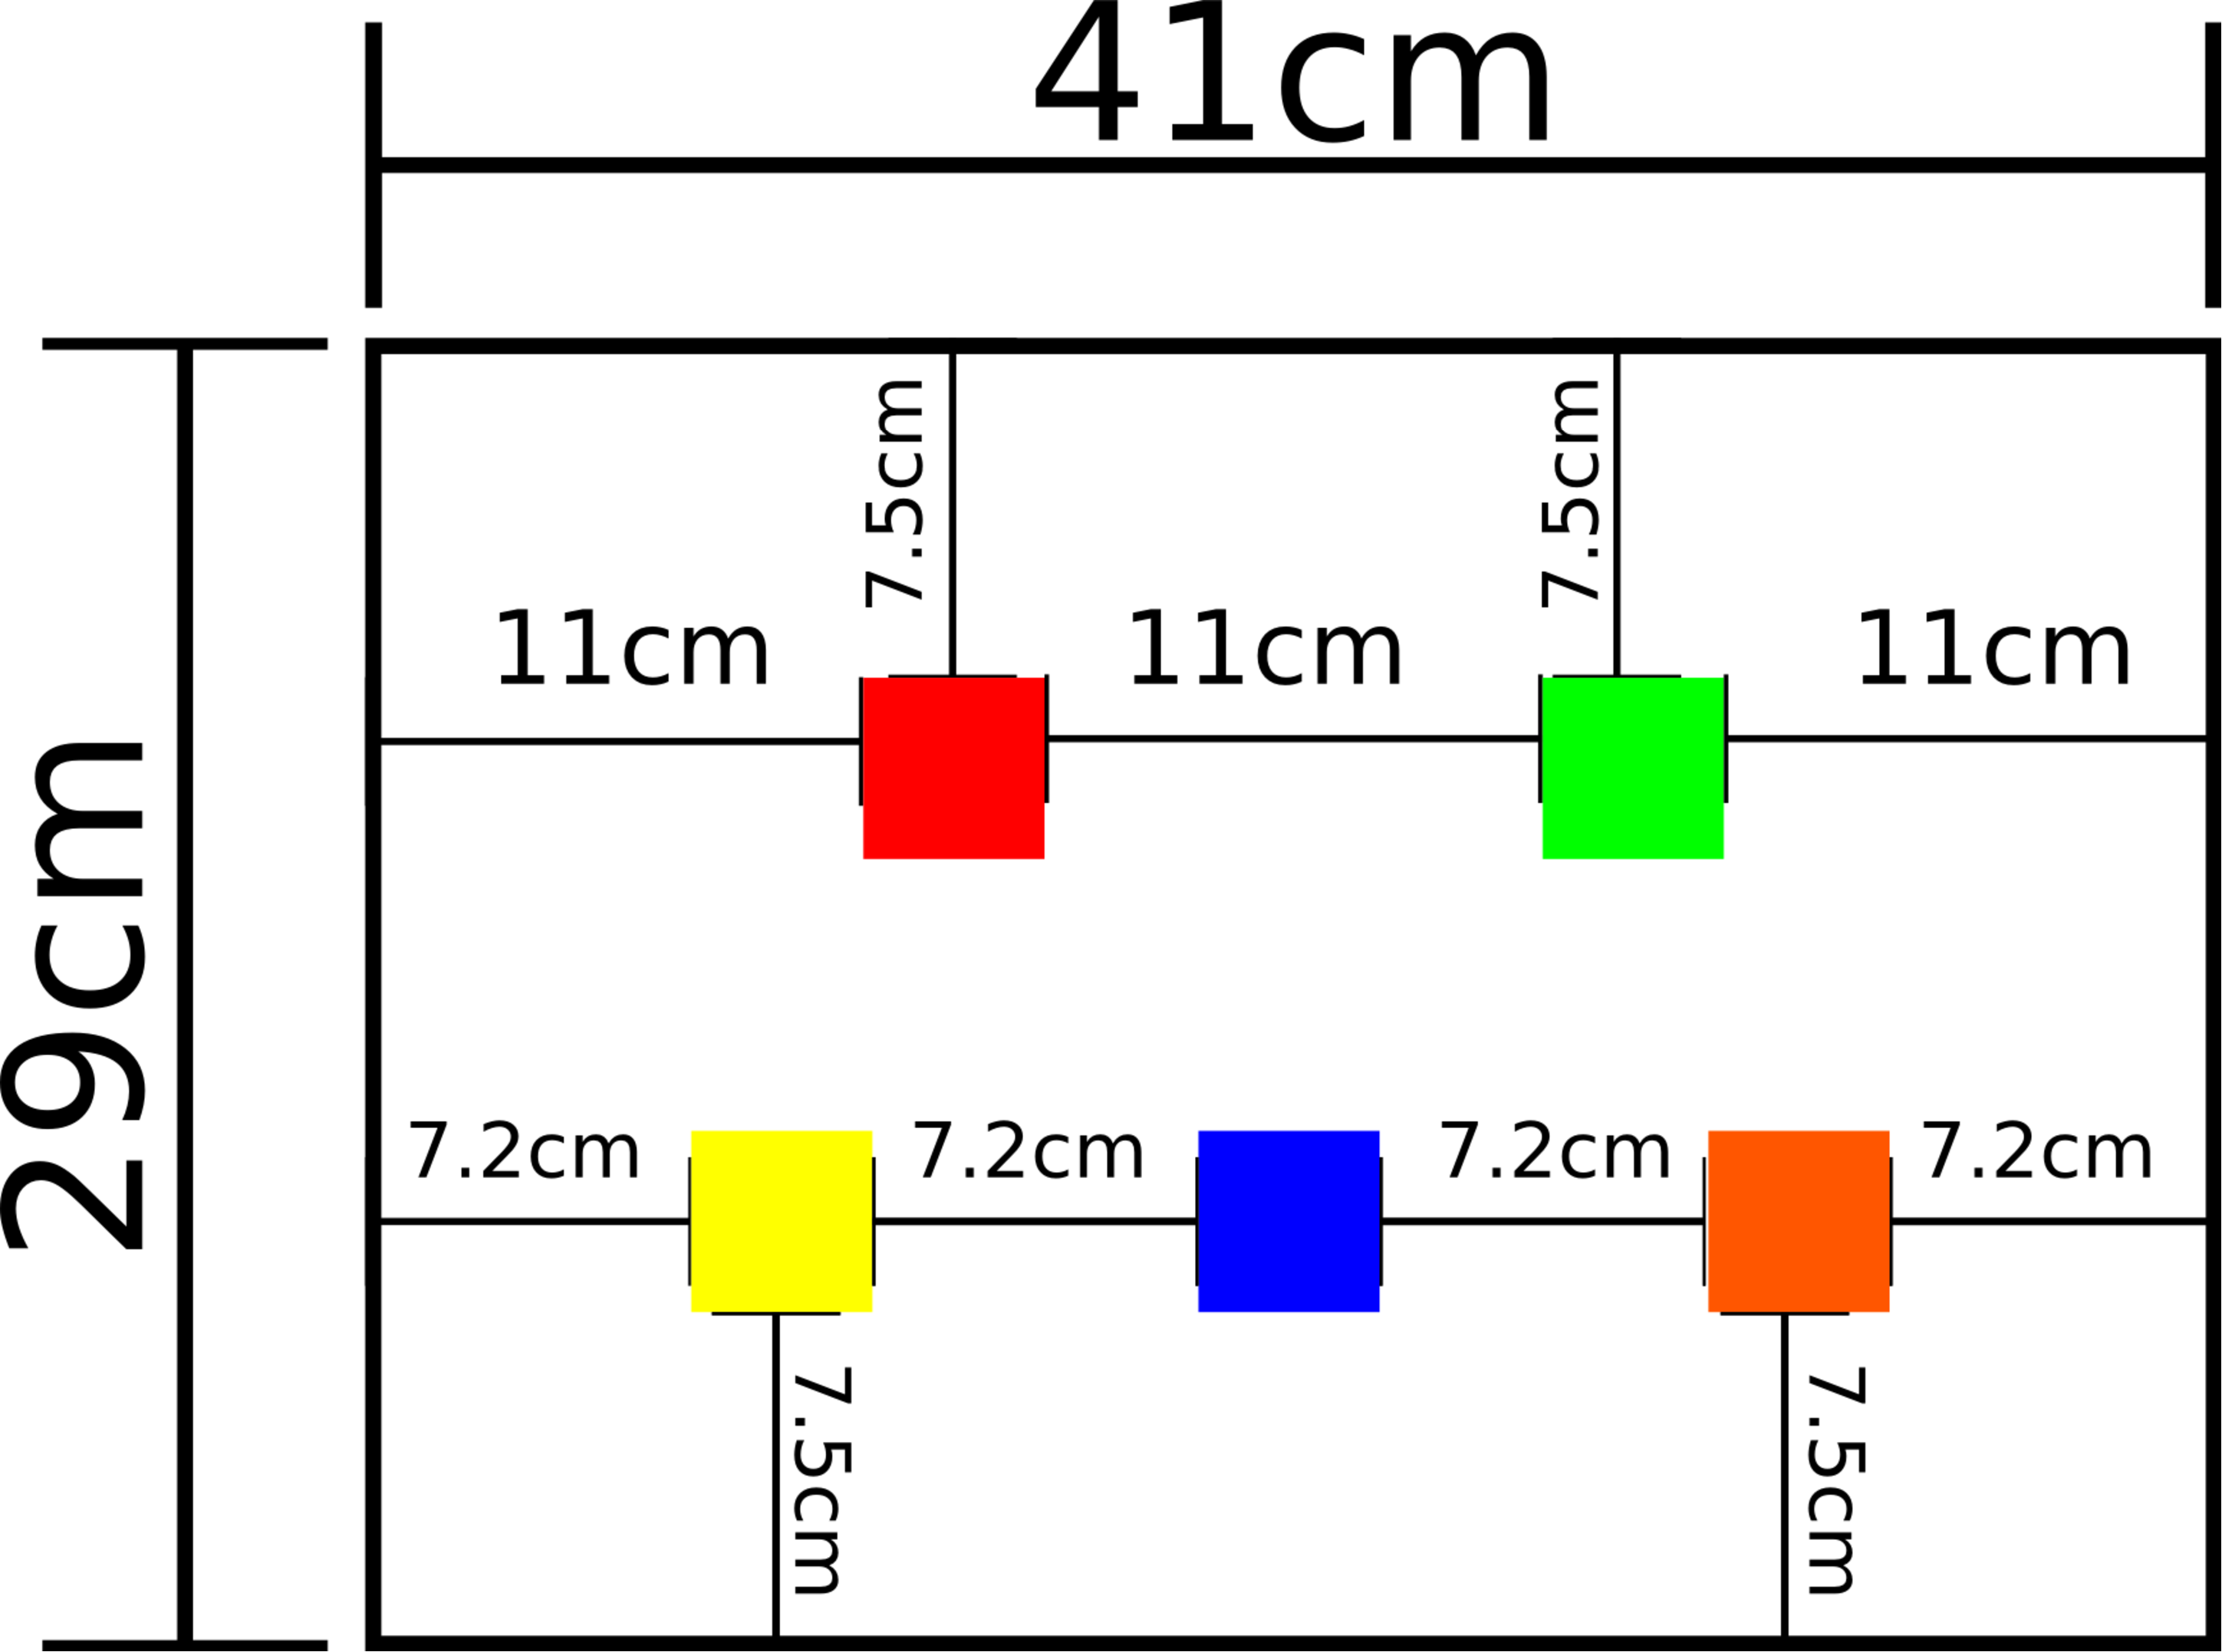
\includegraphics[width=\textwidth]{disposicaoparte.pdf}
\caption{Disposição de cada parte quanto as cores}
\label{fig:figure1}
\end{minipage}
\hspace{0.5cm}
\begin{minipage}[b]{0.45\linewidth}
\centering
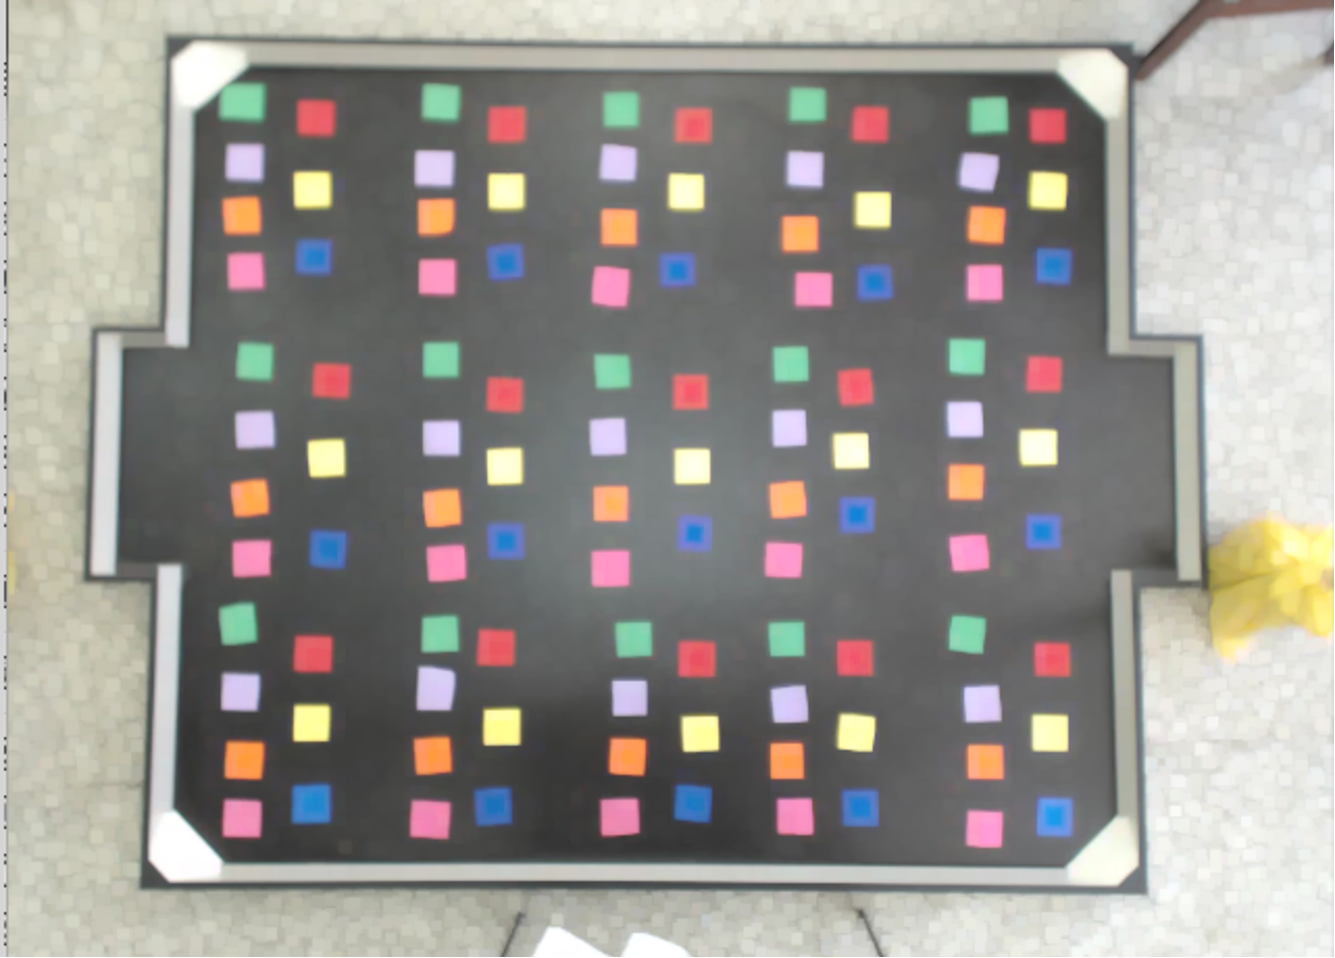
\includegraphics[width=\textwidth]{/testes/campofundo.pdf}
\caption{Campo após terem sido dispostas as cores}
\label{fig:figure2}
\end{minipage}
\end{figure}

\subsection{Cores Comuns}
\subsubsection{Amarelo}
	\begin{figure}[H]
		\centering
		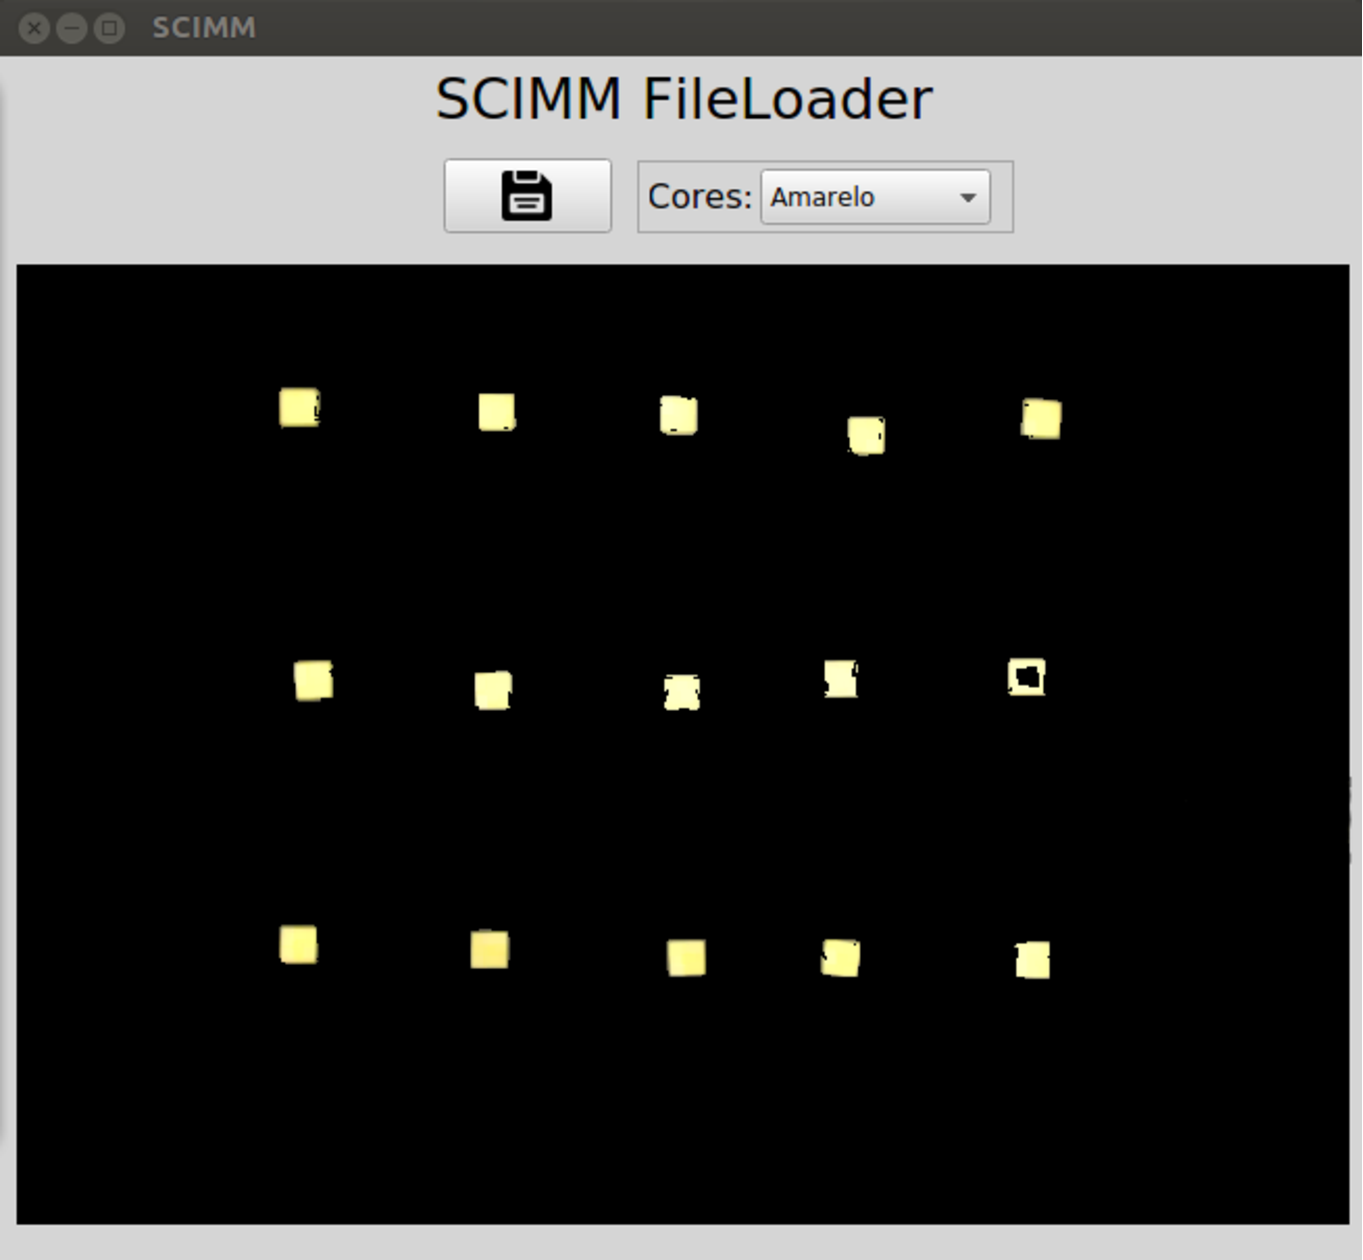
\includegraphics[width=0.5\textwidth]{/testes/amarelo.pdf}
		\caption{Imagem somente com os objetos dentro do intervalo do valor da cor amarela}
		\label{fig:amarelo}
	\end{figure}
	
	Dentre os objetos da cor amarela o sistema encontrou quatorze deles completamente (Figura \ref{fig:amarelo}), e apenas um, que devido a luminosidade implicada em seu centro deixando a tonalidade muito perto do branco, não totalmente preenchido. O detalhamento das quantidades e porcentagem dos objetos encontrador está na Tabela \ref{tab:amarelo}.
	
	\begin{table}[H]
\centering
\begin{tabular}{l|c|c}
Tipo de Objeto & Quantidade & \%  \\% Note a separação de col. e a quebra de linhas
\hline                               % para uma linha horizontal
Objetos Completos & 14 & 93,33 \\
\hline 
Objetos Com Falha de Preenchimento & 1 & 6,66 \\
\hline 
Objetos Com Diminuição de Contorno & 0 &\\
\hline 
Objetos Extrapolados & 0 &\\
\hline 
Objetos Com Diminuição de Área &  0 &\\
\hline 
Objetos Com Falhas Críticas & 0 &\\
\hline 
\end{tabular}
\caption{Categorização Dos Objetos}
\label{tab:amarelo}
\end{table}

Dentre as classificações dos objetos as que descaracterizam o objeto para detecção são: \textit{Objetos Com Falhas Críticas} e \textit{Objetos Com Falha de Preenchimento}, que juntos somam 6,66\% dos objetos.

\subsubsection{Azul}
	\begin{figure}[H]
		\centering
		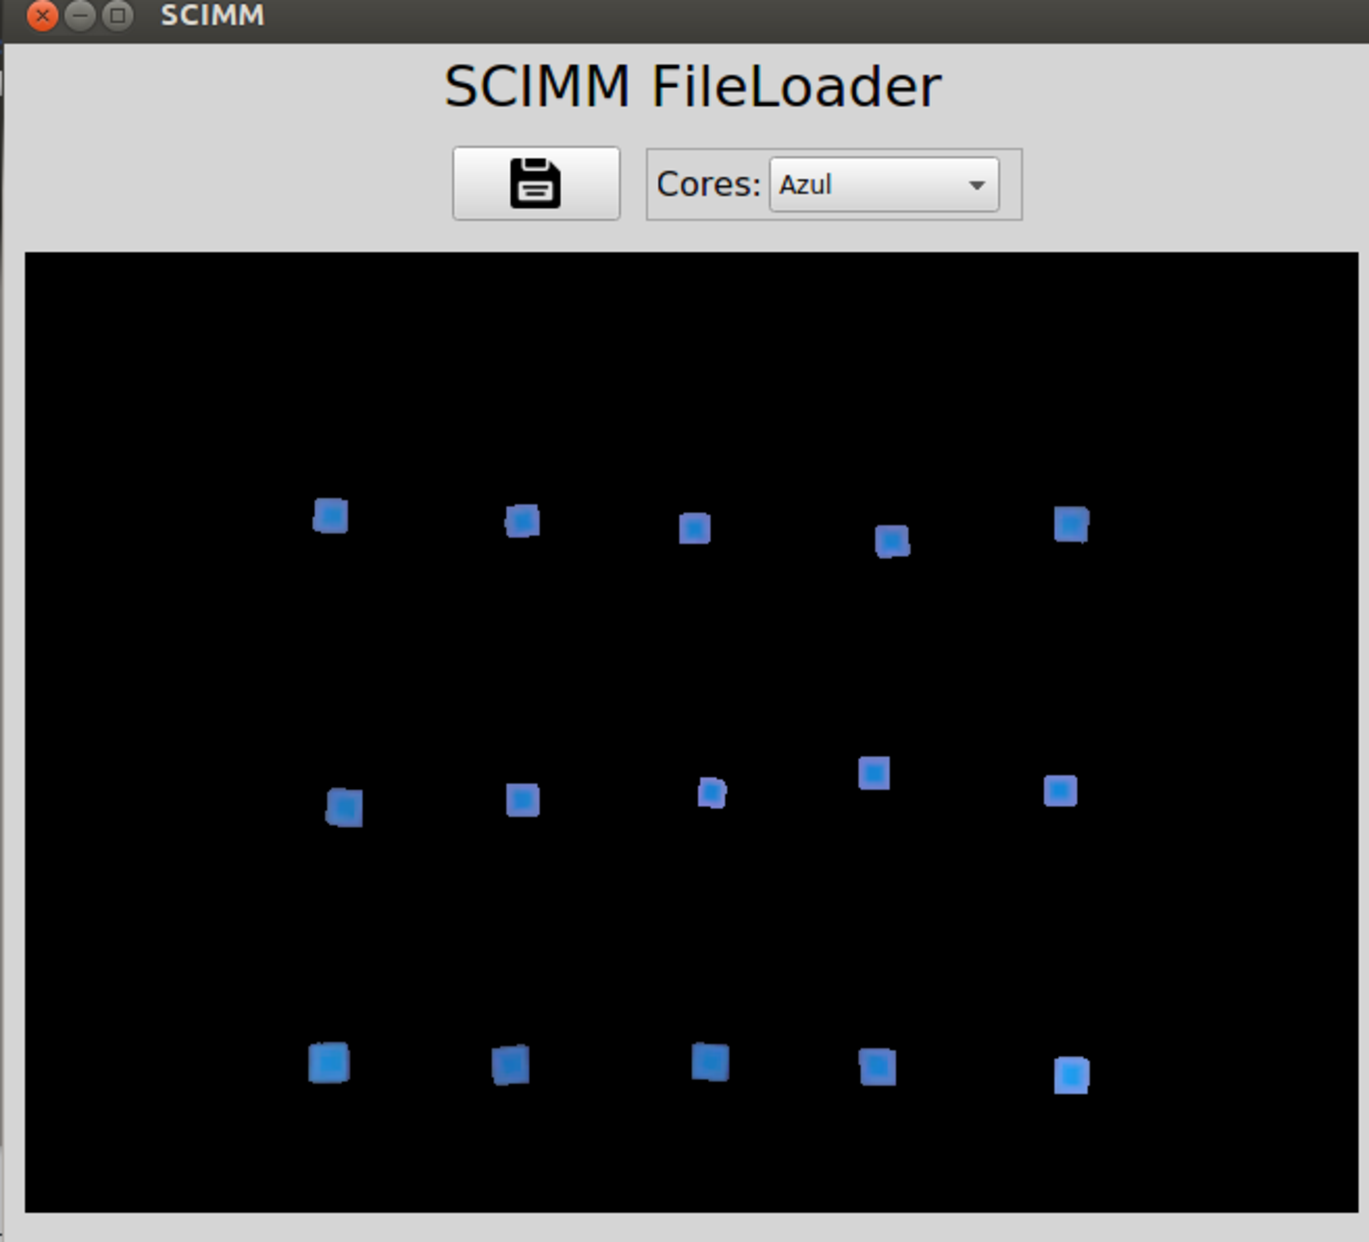
\includegraphics[width=0.5\textwidth]{/testes/azul.pdf}
		\caption{Imagem somente com os objetos dentro do intervalo do valor da cor azul}
		\label{fig:azul}
	\end{figure}

Os objetos da cor azul foram os que obtiveram os melhores resultados, os quinze objetos foram encontrados de forma preenchida. Apesar dos quinze estarem totalmente preenchidos um dos objetos apresentou um tamanho reduzido aos demais devido ao fato de sua borda não ter sido totalmente detectada(Figura \ref{fig:azul}).
O detalhamento das quantidades e porcentagem dos objetos encontrador está na Tabela \ref{tab:azul}.
\begin{table}[h]
\centering
\begin{tabular}{l|c|c}
Tipo de Objeto & Quantidade & \% \\ % Note a separação de col. e a quebra de linhas
\hline                               % para uma linha horizontal
Objetos Completos & 14 & 93,33 \\
\hline 
Objetos Com Falha de Preenchimento & 0\\
\hline 
Objetos Com Diminuição de Contorno &  1 & 6,66
\\
\hline 
Objetos Extrapolados &  0\\
\hline 
Objetos Com Diminuição de Área & 0 \\
\hline 
Objetos Com Falhas Críticas & 0 \\
\hline 
\end{tabular}
\caption{Categorização Dos Objetos}
\label{tab:azul}
\end{table}

\subsubsection{Verde}
\begin{figure}[H]
		\centering
		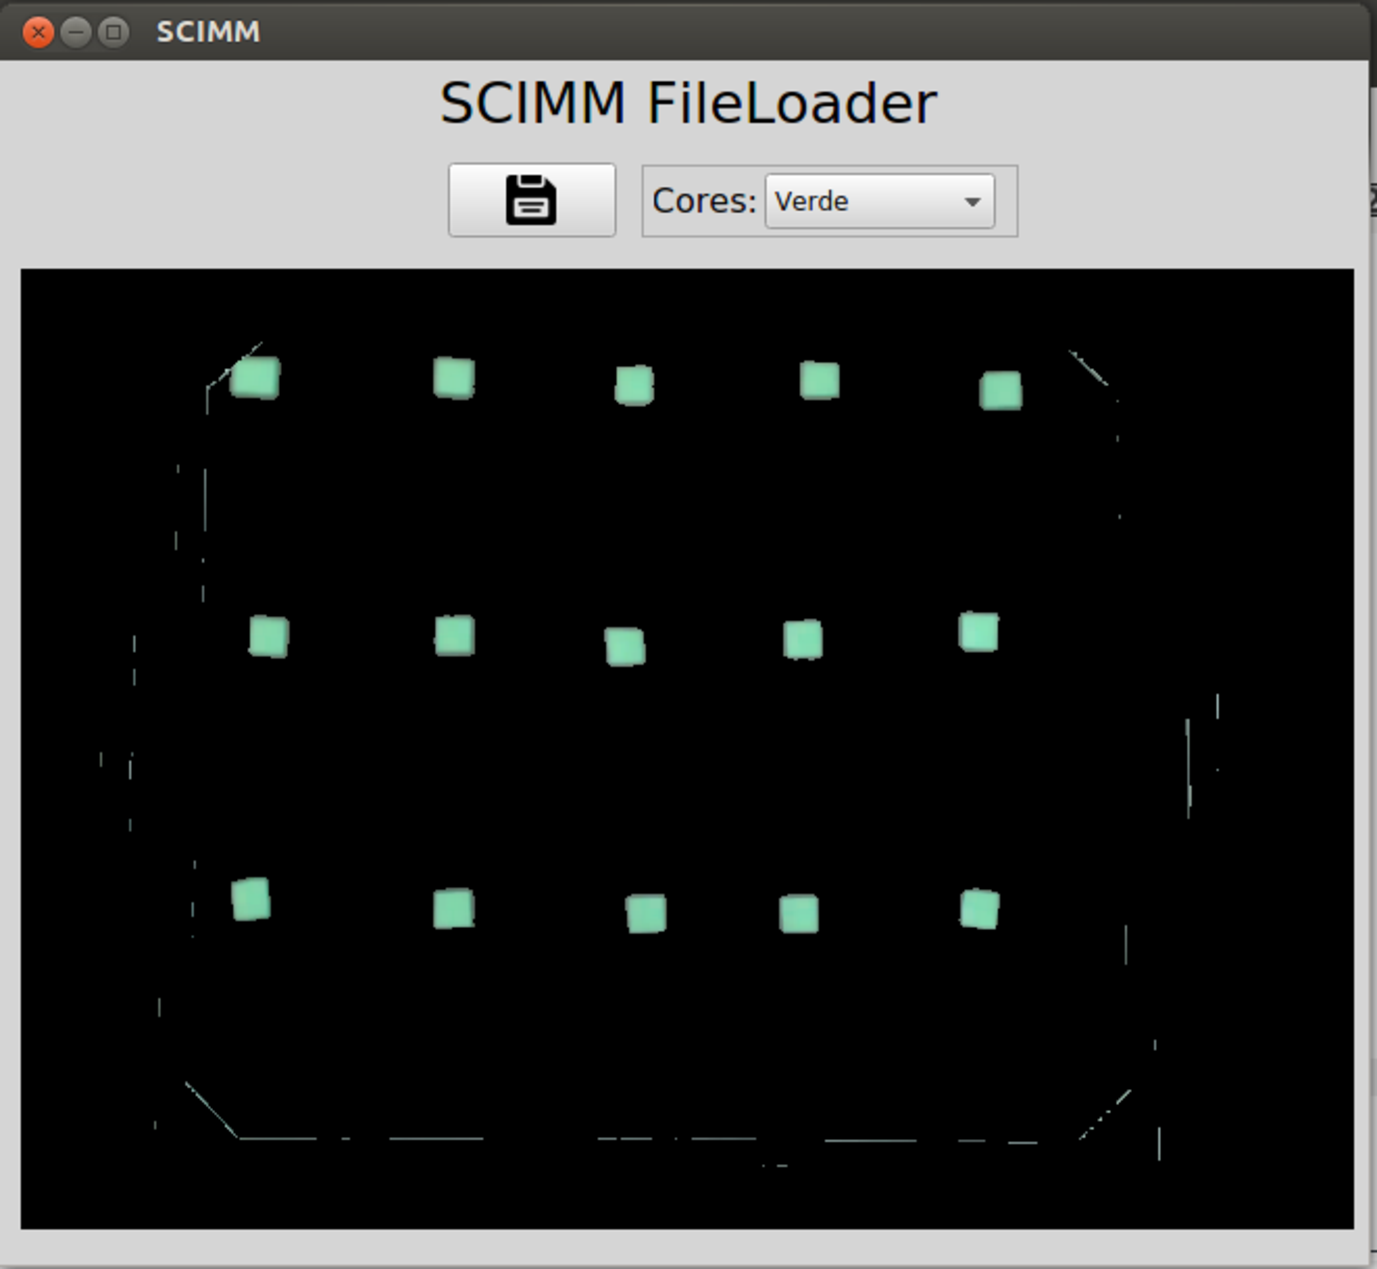
\includegraphics[width=0.5\textwidth]{/testes/verde.pdf}
		\caption{Imagem somente com os objetos dentro do intervalo do valor da cor verde}
		\label{fig:verde}
	\end{figure}

Os objetos da cor verde foram satisfatoriamente encontrados, com seu preenchimento total e não havendo perda de área devido a qualquer interferência de luz em sua borda (Figura \ref{fig:verde}).	
	O detalhamento das quantidades e porcentagem dos objetos encontrador está na Tabela \ref{tab:verde}.
\begin{table}[h]
\centering
\begin{tabular}{l|c|c}
Tipo de Objeto & Quantidade & \% \\ % Note a separação de col. e a quebra de linhas
\hline                               % para uma linha horizontal
Objetos Completos &  15 &100 \\
\hline 
Objetos Com Falha de Preenchimento & 0\\
\hline 
Objetos Com Diminuição de Contorno &  0\\
\hline 
Objetos Extrapolados & 0 \\
\hline 
Objetos Com Diminuição de Área &  0 \\
\hline 
Objetos Com Falhas Críticas & 0 \\
\hline 
\end{tabular}
\caption{Categorização Dos Objetos}
\label{tab:verde}
\end{table}	
\subsubsection{Rosa}
	
	\begin{figure}[H]
		\centering
		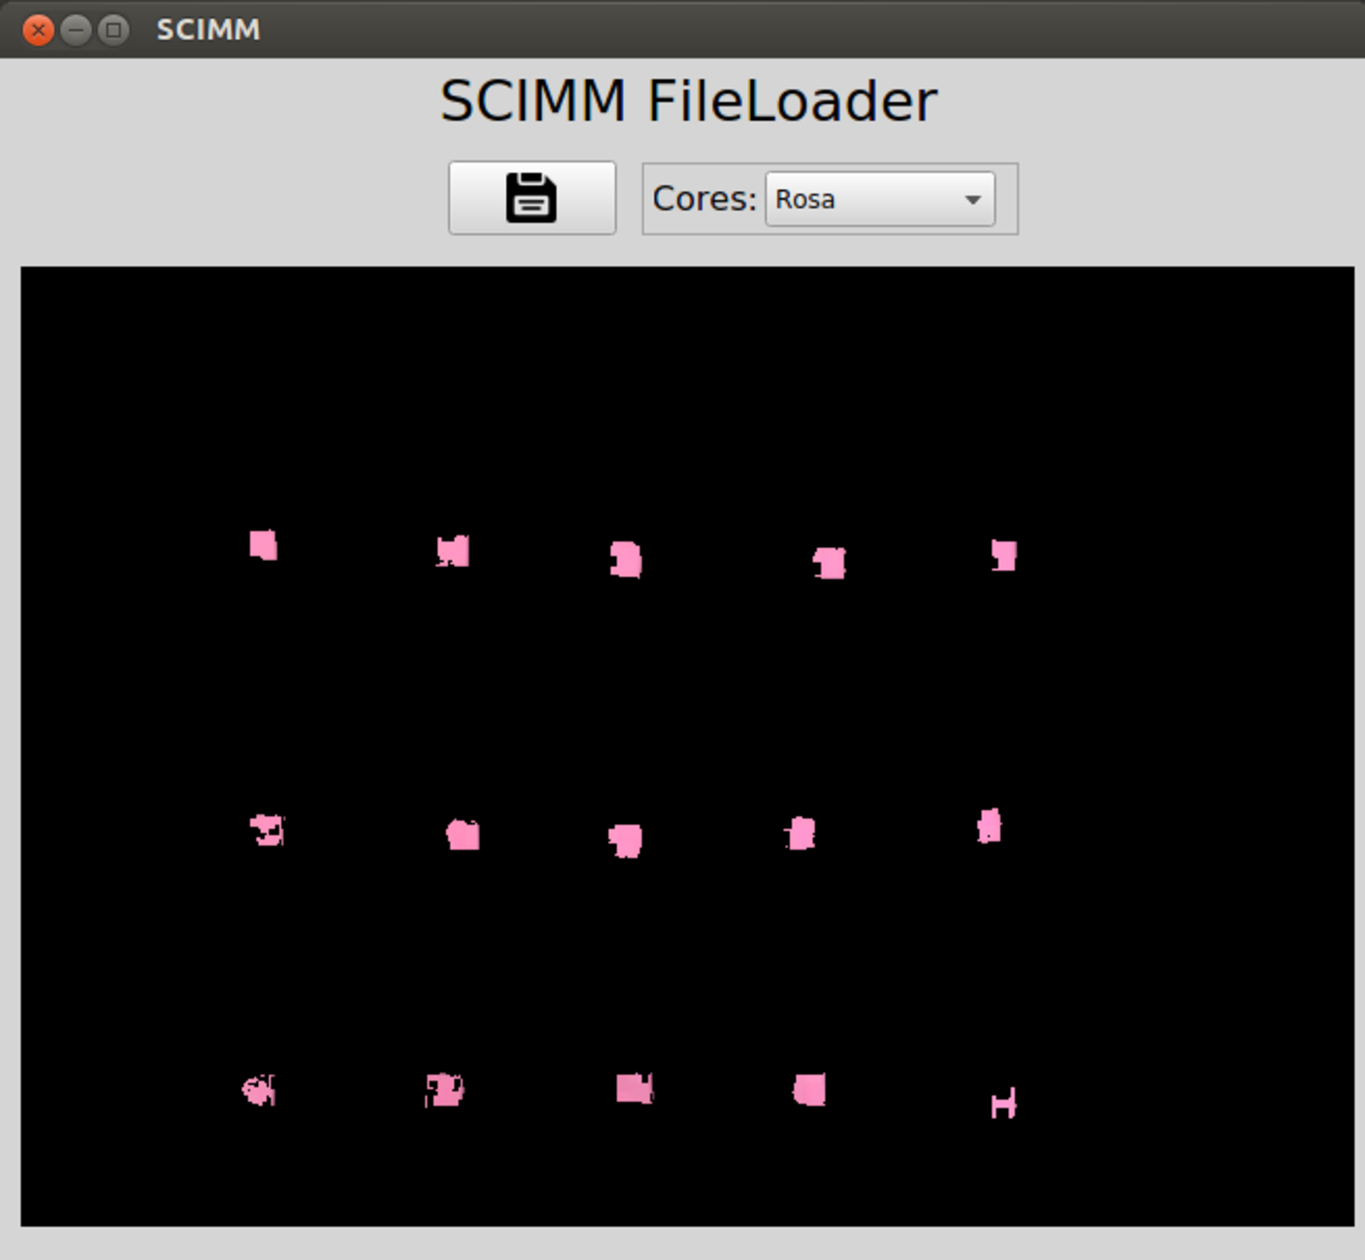
\includegraphics[width=0.5\textwidth]{/testes/rosa.pdf}
		\caption{Imagem somente com os objetos dentro do intervalo do valor da cor rosa}
		\label{fig:rosa}
	\end{figure}
	
Dentre os objetos Rosa detectados, quatro obtiveram falhas em sua detecção, falhas de preenchimento e diminuição de borda, sendo desconsiderados. Dentro os outros onze: três foram detectados sem falhas de preenchimentos apenas com diminuição de área, para aproximadamente metade da área real do objeto; os outros oito foram encontrados apenas com diminuição de área, devido a diminuição de borda(Figura \ref{fig:rosa}).  O detalhamento das quantidades e porcentagem dos objetos encontrador está na Tabela \ref{tab:rosa},
	
	\begin{table}[h]
\centering
\begin{tabular}{l|c|c}
Tipo de Objeto & Quantidade  & \% \\ % Note a separação de col. e a quebra de linhas
\hline                               % para uma linha horizontal
Objetos Completos &  0\\
\hline 
Objetos Com Falha de Preenchimento & 0\\
\hline 
Objetos Com Diminuição de Contorno & 8& 53,33
 \\
\hline 
Objetos Extrapolados & 0 \\
\hline 
Objetos Com Diminuição de Área & 3 & 20\\
\hline 
Objetos Com Falhas Críticas & 4 & 26,66 \\
\hline 
\end{tabular}
\caption{Categorização Dos Objetos}
\label{tab:rosa}
\end{table}

Dentre as classificações dos objetos as que descaracterizam o objeto para detecção são:  \textit{Objetos Com Falhas Críticas} e \textit{Objetos Com Falha de Preenchimento} que juntos somam 26,66\% dos objetos. Apesar de ser um numero não tão baixo, a cor rosa não é uma cor que a equipe Cedro costuma usar em seus jogos, sendo assim, essa taxa de erro não influencia na eficiência do sistema.
\subsubsection{Roxo}
\begin{figure}[H]
		\centering
		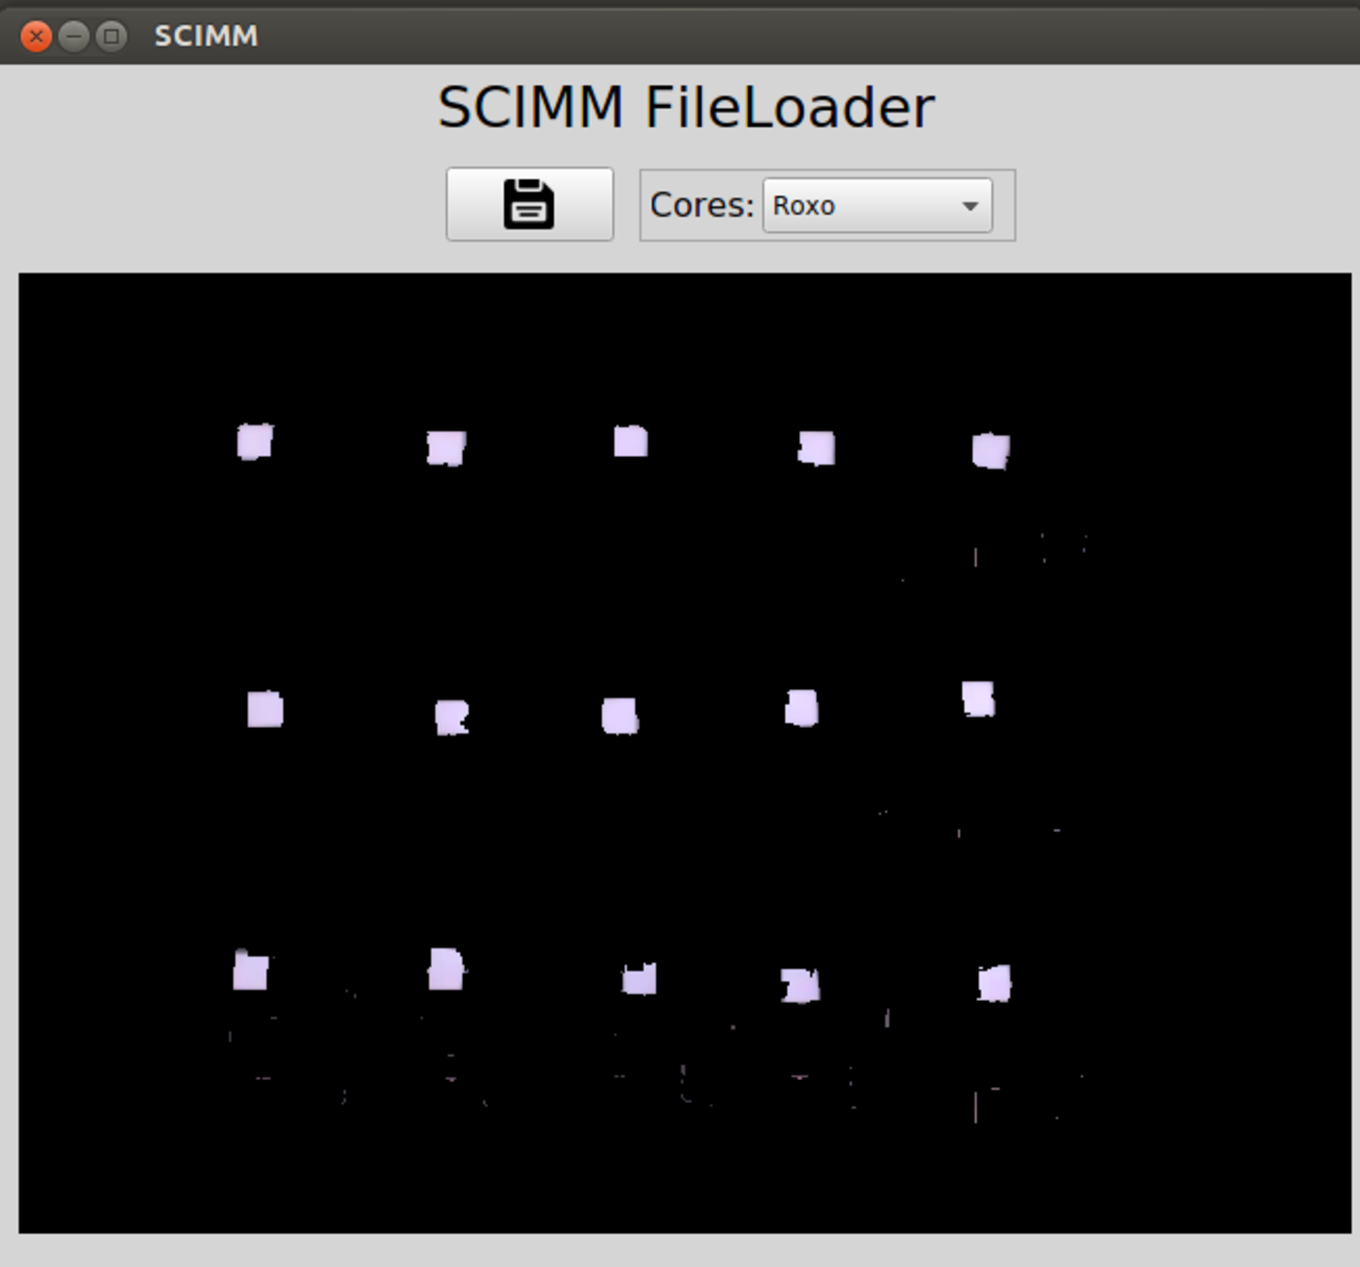
\includegraphics[width=0.5\textwidth]{/testes/roxo.pdf}
		\caption{Imagem somente com os objetos dentro do intervalo do valor da cor roxo}
		\label{fig:roxo}
	\end{figure}

Todos os objetos roxos dispostos no campo foram encontrados pelo intervalo da cor(Figura \ref{fig:roxo}). Dentre os quinze, quatro não apresentaram problema algum e foram completamente detectados; oito possuíram diminuição em seu contorno e três apresentaram diminuição de área. O detalhamento das quantidades e porcentagem dos objetos encontrador está na Tabela \ref{tab:roxo}.
\begin{table}[H]
\centering
\begin{tabular}{l|c|c}
Tipo de Objeto & Quantidade  & \% \\ % Note a separação de col. e a quebra de linhas
\hline                               % para uma linha horizontal
Objetos Completos &  4 & 26,66\\
\hline 
Objetos Com Falha de Preenchimento & 0 \\
\hline 
Objetos Com Diminuição de Contorno &  8 & 53,33\\
\hline 
Objetos Extrapolados & 0 \\
\hline 
Objetos Com Diminuição de Área & 3 & 20\\
\hline 
Objetos Com Falhas Críticas & 0 \\
\hline 
\end{tabular}
\caption{Categorização Dos Objetos}
\label{tab:roxo}
\end{table}
	
\subsection{Cores Com Problemas Conhecidos}
Cores como Vermelho e Laranja possuem o problema de por vezes, devido a interferência externa, se assemelharem a outras. Este problemas já são de conhecimento da área.
	
	
\subsubsection{Vermelho}
	\begin{figure}[H]
		\centering
		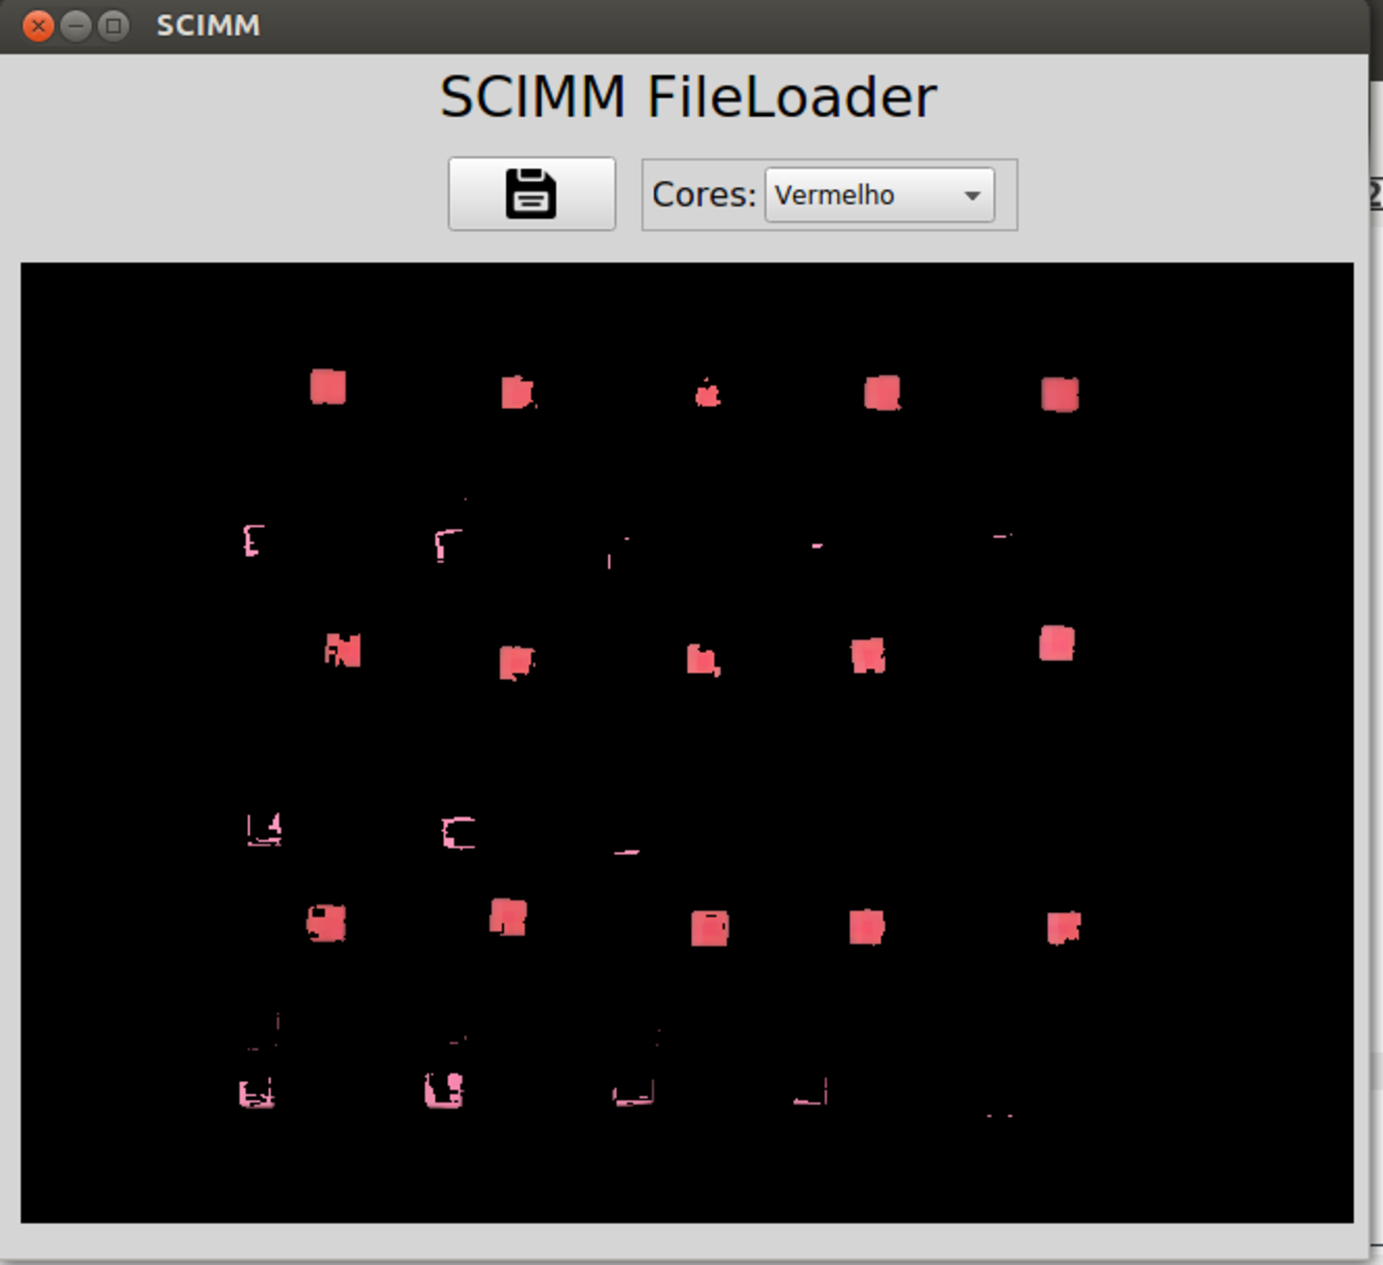
\includegraphics[width=0.5\textwidth]{/testes/vermelho.pdf}
		\caption{Imagem somente com os objetos dentro do intervalo do valor da cor vermelho}
		\label{fig:vermelho}
	\end{figure}

A cor rosa, em determinadas luminosidades pode acabar sendo semelhante a cor vermelha, por este motivo, alguns traços dos objetos rosas estão aparecendo dentro do intervalo de calibração(Figura \ref{fig:vermelho}). Porem serão ignorados, uma vez que é possível ser feito a separação das cores via software.	

Dentre as classificações dos objetos as que 
descaracterizam o objeto para detecção são: \textit{Objetos Com Falhas Críticas} e \textit{Objetos Com Falha de Preenchimento} que juntos somam somente 13,32\% dos objetos. A quantidade e porcentagem dos demais objetos podem ser vistas na Tabela \ref{tab:vermelho}.
	
	\begin{table}[h]
\centering
\begin{tabular}{l|c|c}
Tipo de Objeto & Quantidade  & \% \\ % Note a separação de col. e a quebra de linhas
\hline                               % para uma linha horizontal
Objetos Completos &  8 & 53,33 \\
\hline 
Objetos Com Falha de Preenchimento & 1 & 6,66 \\
\hline 
Objetos Com Diminuição de Contorno &  4 & 26,66 \\
\hline 
Objetos Extrapolados &  13 \\
\hline 
Objetos Com Diminuição de Área &  1 &6,66 \\
\hline 
Objetos Com Falhas Críticas &  1 & 6,66\\
\hline 
\end{tabular}
\caption{Categorização Dos Objetos}
\label{tab:vermelho}
\end{table}



\subsubsection{Laranja}
	\begin{figure}[H]
		\centering
		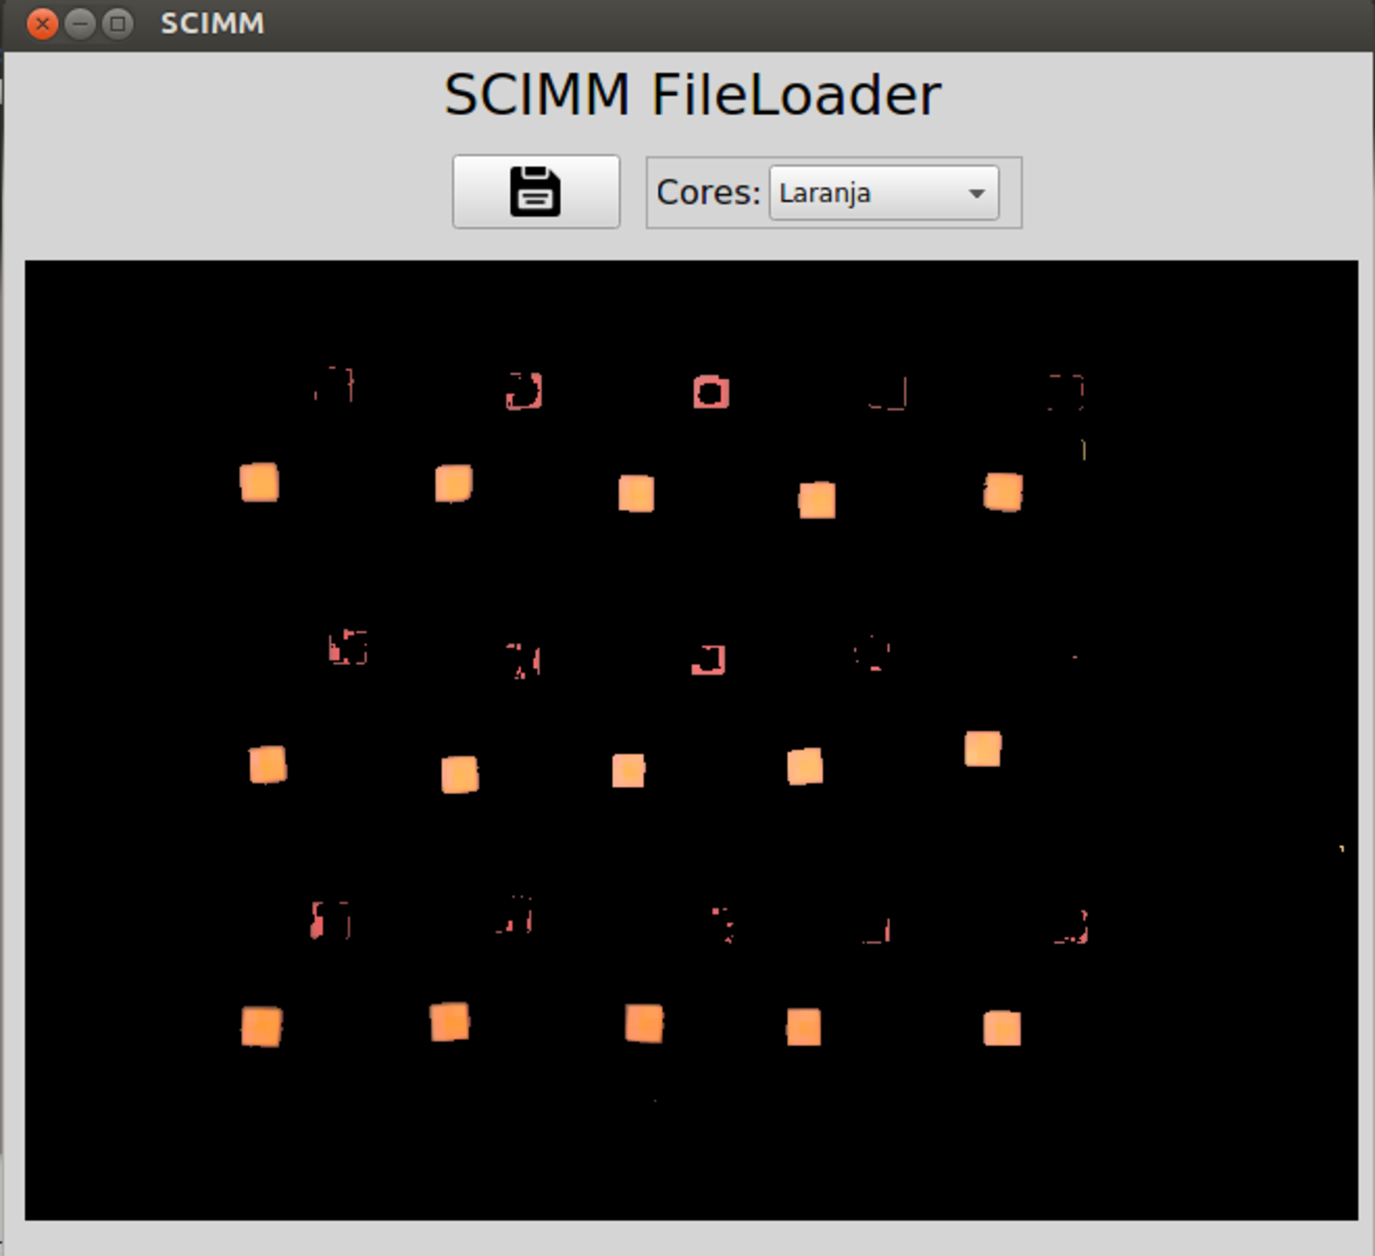
\includegraphics[width=0.5\textwidth]{/testes/laranja.pdf}
		\caption{Imagem somente com os objetos dentro do intervalo do valor da cor laranja}
		\label{fig:laranja}
	\end{figure}
	
	Devido à um problema muito comum na área de calibração de cores, a cor laranja possui o problema de ser, por muitas vezes, semelhante a vermelha(Figura \ref{fig:laranja}). Devido a luminosidade implicada tanto em uma quanto na outra, ambas as cores tendem a se tornarem próximas.
	Sabendo deste problema, o fato de terem sido encontrados objetos da cor vermelha dentro do intervalo de valores da cor laranja é ignorado e somente serão levados em consideração os objetos visualmente laranjas.
	Os quinze objetos da cor laranja foram encontrados com precisão. Todos possuindo seu completo preenchimento e borda. As quantidade e porcentagens do objetos estão disposto na Tabela \ref{tab:laranja}.
	
\begin{table}[h]
\centering
\begin{tabular}{l|c|c}
Tipo de Objeto & Quantidade  & \% \\ % Note a separação de col. e a quebra de linhas
\hline                               % para uma linha horizontal
Objetos Completos &  15 & 100 \\
\hline 
Objetos Com Falha de Preenchimento & 0 \\
\hline 
Objetos Com Diminuição de Contorno &  0 \\
\hline 
Objetos Extrapolados & 8 \\
\hline 
Objetos Com Diminuição de Área &  0 \\
\hline 
Objetos Com Falhas Críticas & 0 \\
\hline 
\end{tabular}
\caption{Categorização Dos Objetos}
\label{tab:laranja}
\end{table}
\newpage
\subsection{Analise Geral}
De modo total estavam disposto pelo campo 105 objetos coloridos, pode ser visto na Figura \ref{fig:total} a quantidade de objetos que se encontram em cada uma das categorias. Destes, 66,7\% dos objetos foram encontrados corretamente, 1,9\% foram encontrados com falhas de preenchimento, 20\% apresentaram perda de contorno, 6,67\% apresentaram diminuição da área e 4,76\% apresentaram falhas e faltas que prejudicaram totalmente o objeto.
	\begin{figure}[H]
		\centering
		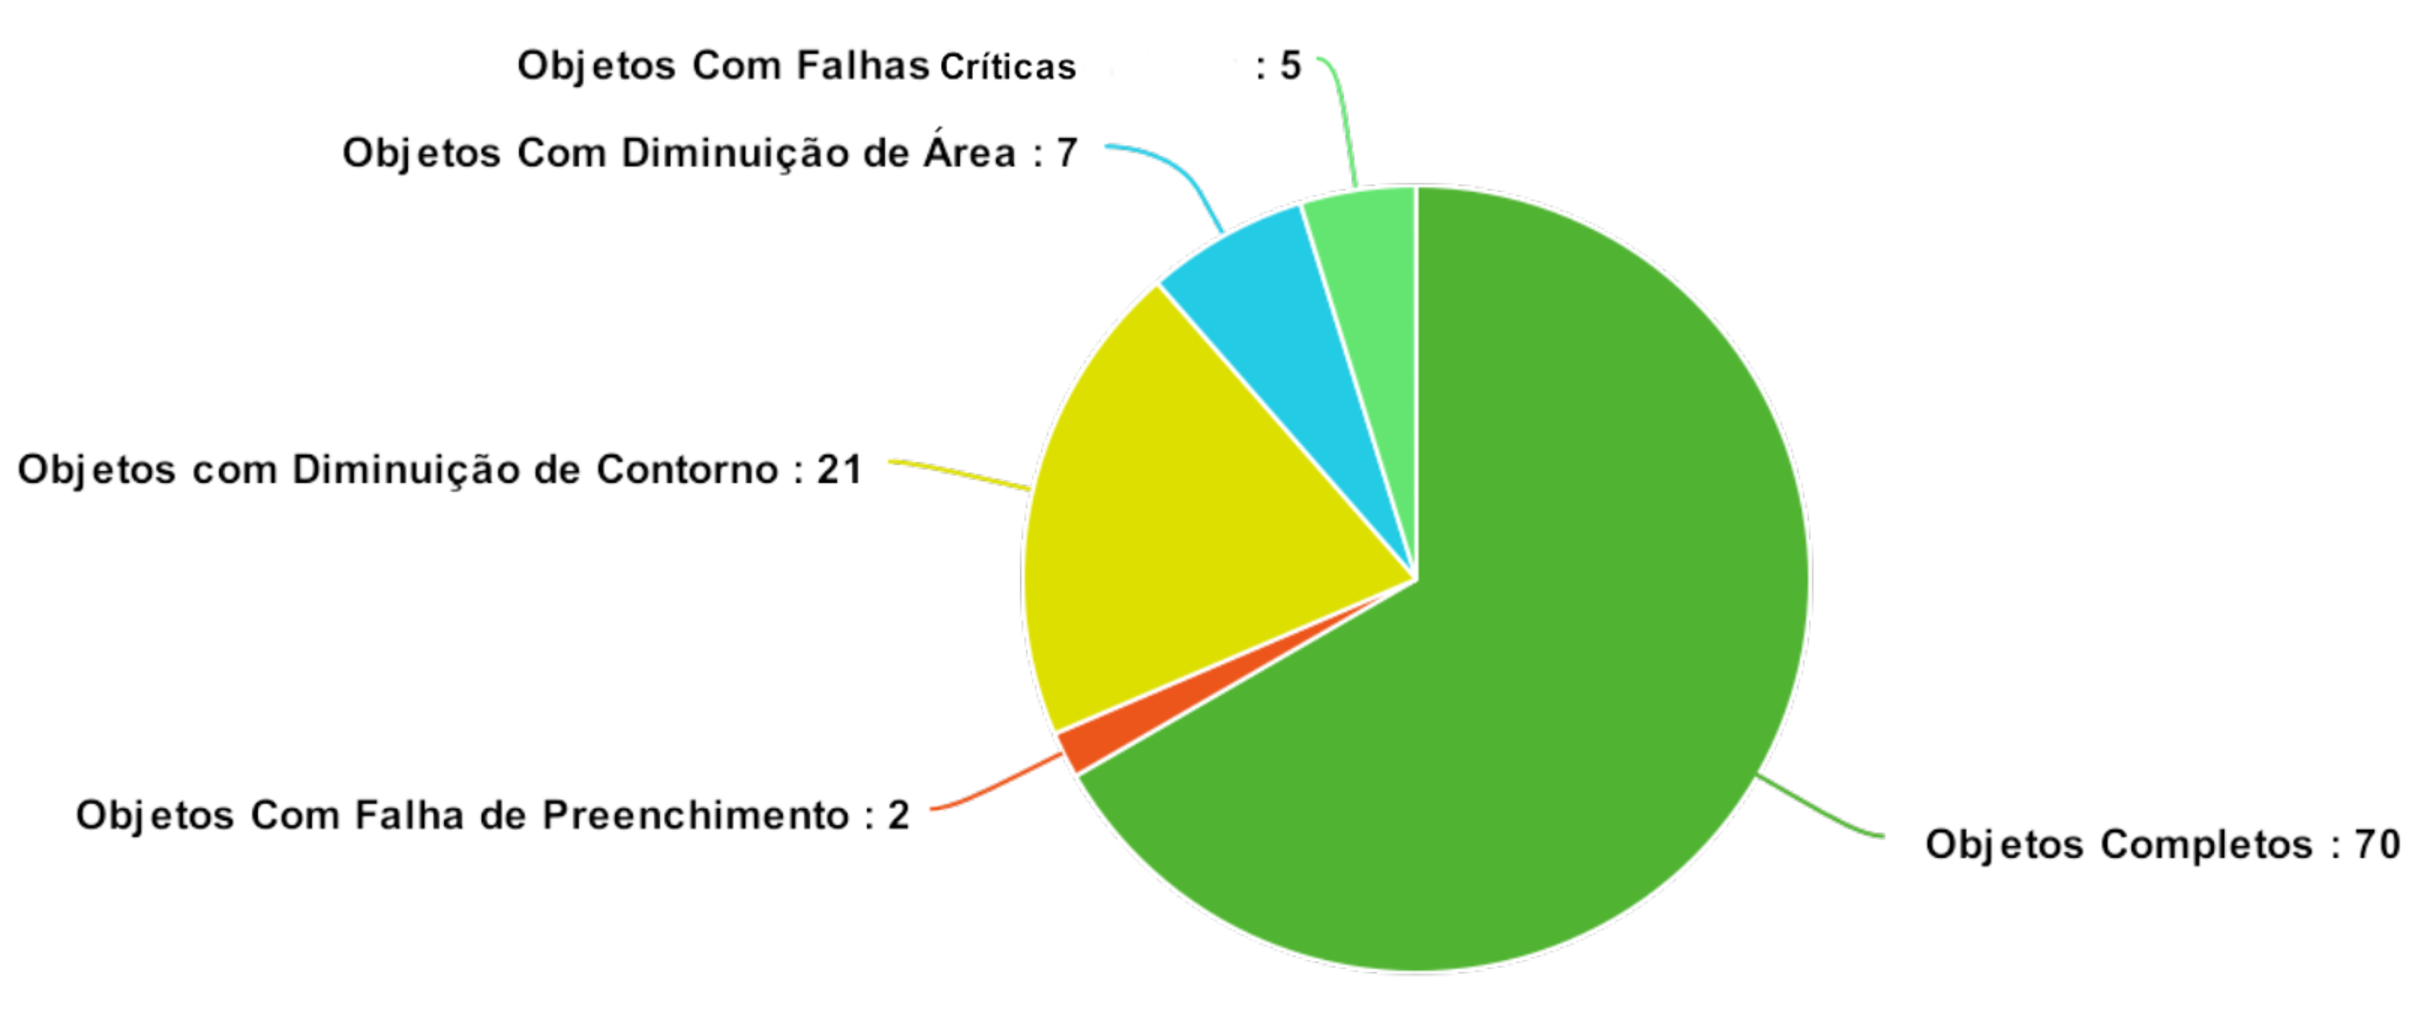
\includegraphics[width=0.8\textwidth]{/testes/graficotestes.pdf}
		\caption{Gráfico de análise do resultado dos testes}
		\label{fig:total}
	\end{figure}
	
	
	Sabendo destes valores, os que podem ser considerados críticos na detecção de objetos por meio da sua cor são \textit{Objetos Com Falhas Críticas} e \textit{Objetos Com Falha de Preenchimento} que juntos somam 6,67\% dos objetos.
	
	\section{Considerações Finais}
	
	Pode-se concluir que o sistema SCIMM apresentou ótimos resultado com as cores amarelo, azul, laranja e verde, resultados bons com a cor vermelha, e resultados satisfatório com a cor roxo, no entanto obteve um resultado ruim com a cor rosa. 
	
	As cores calibradas pelo sistema, quando testadas em ambiente de detecção de objetos coloridos, simbolizaram 98 dos 105 objetos, conseguindo com que somente 7 objetos coloridos não tenham sido identificados.